\documentclass[10pt,a4paper]{article}
\usepackage{admos-article}

% ---------- Article information: edit this block ----------
\newcommand{\ArticleType}{TECHNICAL ARTICLE}
\newcommand{\ArticleSeries}{Low-Frequency Noise}
\newcommand{\ArticleID}{LFN-002}
\newcommand{\ArticleDate}{25.10.2026}
\newcommand{\ArticleTitle}{Beyond the 1/f spectrum: Influence of flicker noise on RF Circuits}
\newcommand{\ArticleSubtitle}{Low-Frequency Noise in High-Frequency Circuits}
\newcommand{\ArticleTags}{
Tag1,
Tag2,
Tag3,
Tag4,
TAg5,
}

\begin{document}
	
	\pagestyle{empty}
	
	% ============================================================
	% PAGE 1 START
	% ============================================================
	
	\ArticleMetadata
	\ArticleTitleBlock
	
	Low-frequency noise is often associated with slowly varying
	electrical fluctuations, seemingly far removed from the
	operating frequencies of modern analog and RF circuits.
	However, its influence is not necessarily confined to
	the low-frequency spectrum. Through nonlinear and
	time-varying circuit behavior, flicker noise can be
	translated to higher frequencies, affecting the performance
	of circuits operating in the megahertz and gigahertz
	regimes. In oscillators, it contributes to close-in phase
	noise, while in mixers and precision analog circuits, it
	can limit signal integrity and resolution. Understanding
	how these low-frequency fluctuations manifest at the
	circuit level is therefore essential for designing
	high-performance analog and RF systems.
	

	
	\begin{figure}[htbp]
		   \centering
		  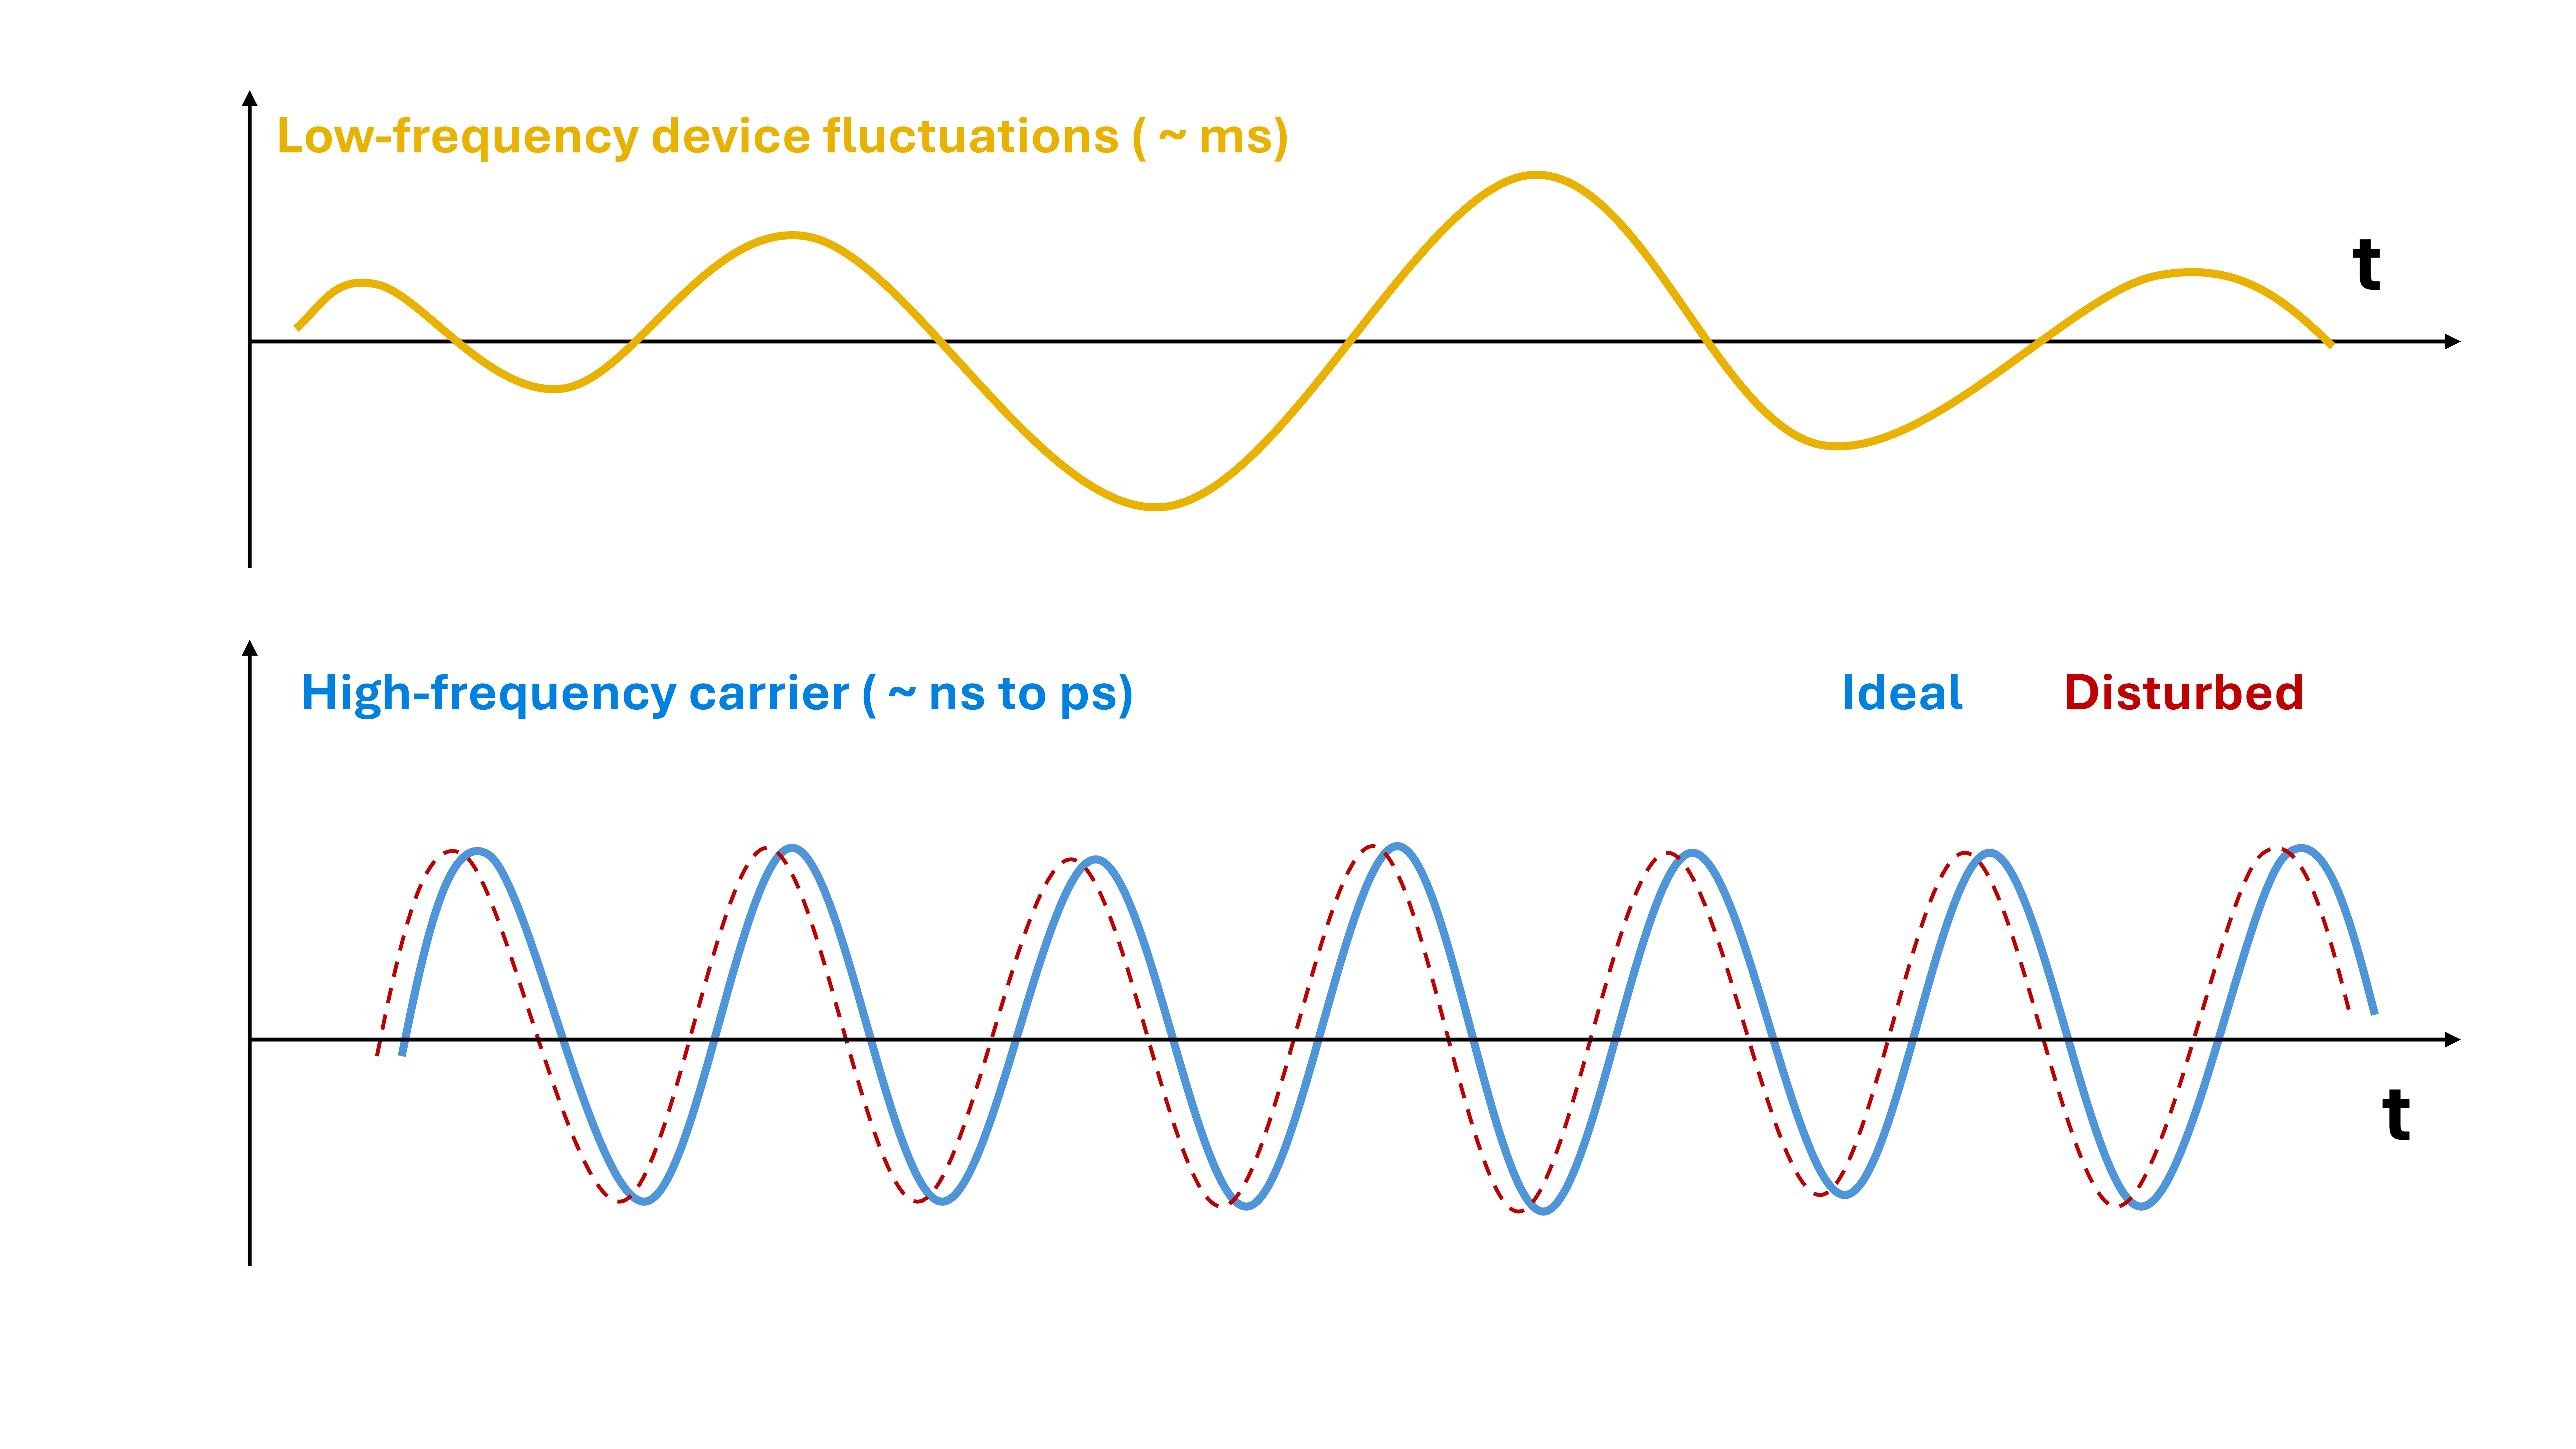
\includegraphics[width=0.52\linewidth]{figures/fig1.png}
		   \caption{
			    Slowly varying device fluctuations occurring over millisecond timescales can perturb the phase of a high-frequency carrier oscillating on nanosecond or picosecond timescales.
			  }
		   \label{fig:fig1}
	 \end{figure}
	
	\section{The Principle of Noise Upconversion}
	
	In a linear, time-invariant circuit, noise components retain
	their original frequencies, although their amplitudes may
	change. However, many analog and RF circuits operate under
	nonlinear or periodically time-varying conditions, enabling
	noise to be transferred between different frequency regions.
	This phenomenon, commonly referred to as noise frequency
	conversion or upconversion, explains how low-frequency
	fluctuations can influence signals operating at much higher
	frequencies.
	
	Consider a transistor operating within an RF circuit.
	Slow fluctuations in its electrical characteristics, such
	as drain current, transconductance, or effective capacitance,
	can interact with the high-frequency signal. Depending on
	the circuit architecture, these fluctuations may modulate
	the amplitude, phase, or instantaneous frequency of the
	carrier \cite{Hajimiri1998}.
	
	The frequency-domain interpretation of noise upconversion
	is illustrated in Figure~\ref{fig:fig2}. The characteristic
	$1/f$-like noise spectrum, with increasing power spectral
	density (PSD) toward lower frequencies near DC, can be translated
	to frequencies around a high-frequency carrier through
	nonlinear or time-varying circuit behavior. The resulting
	noise sidebands appear on either side of the carrier,
	potentially degrading its spectral purity.
	
	\begin{figure}[htbp]
		\centering
		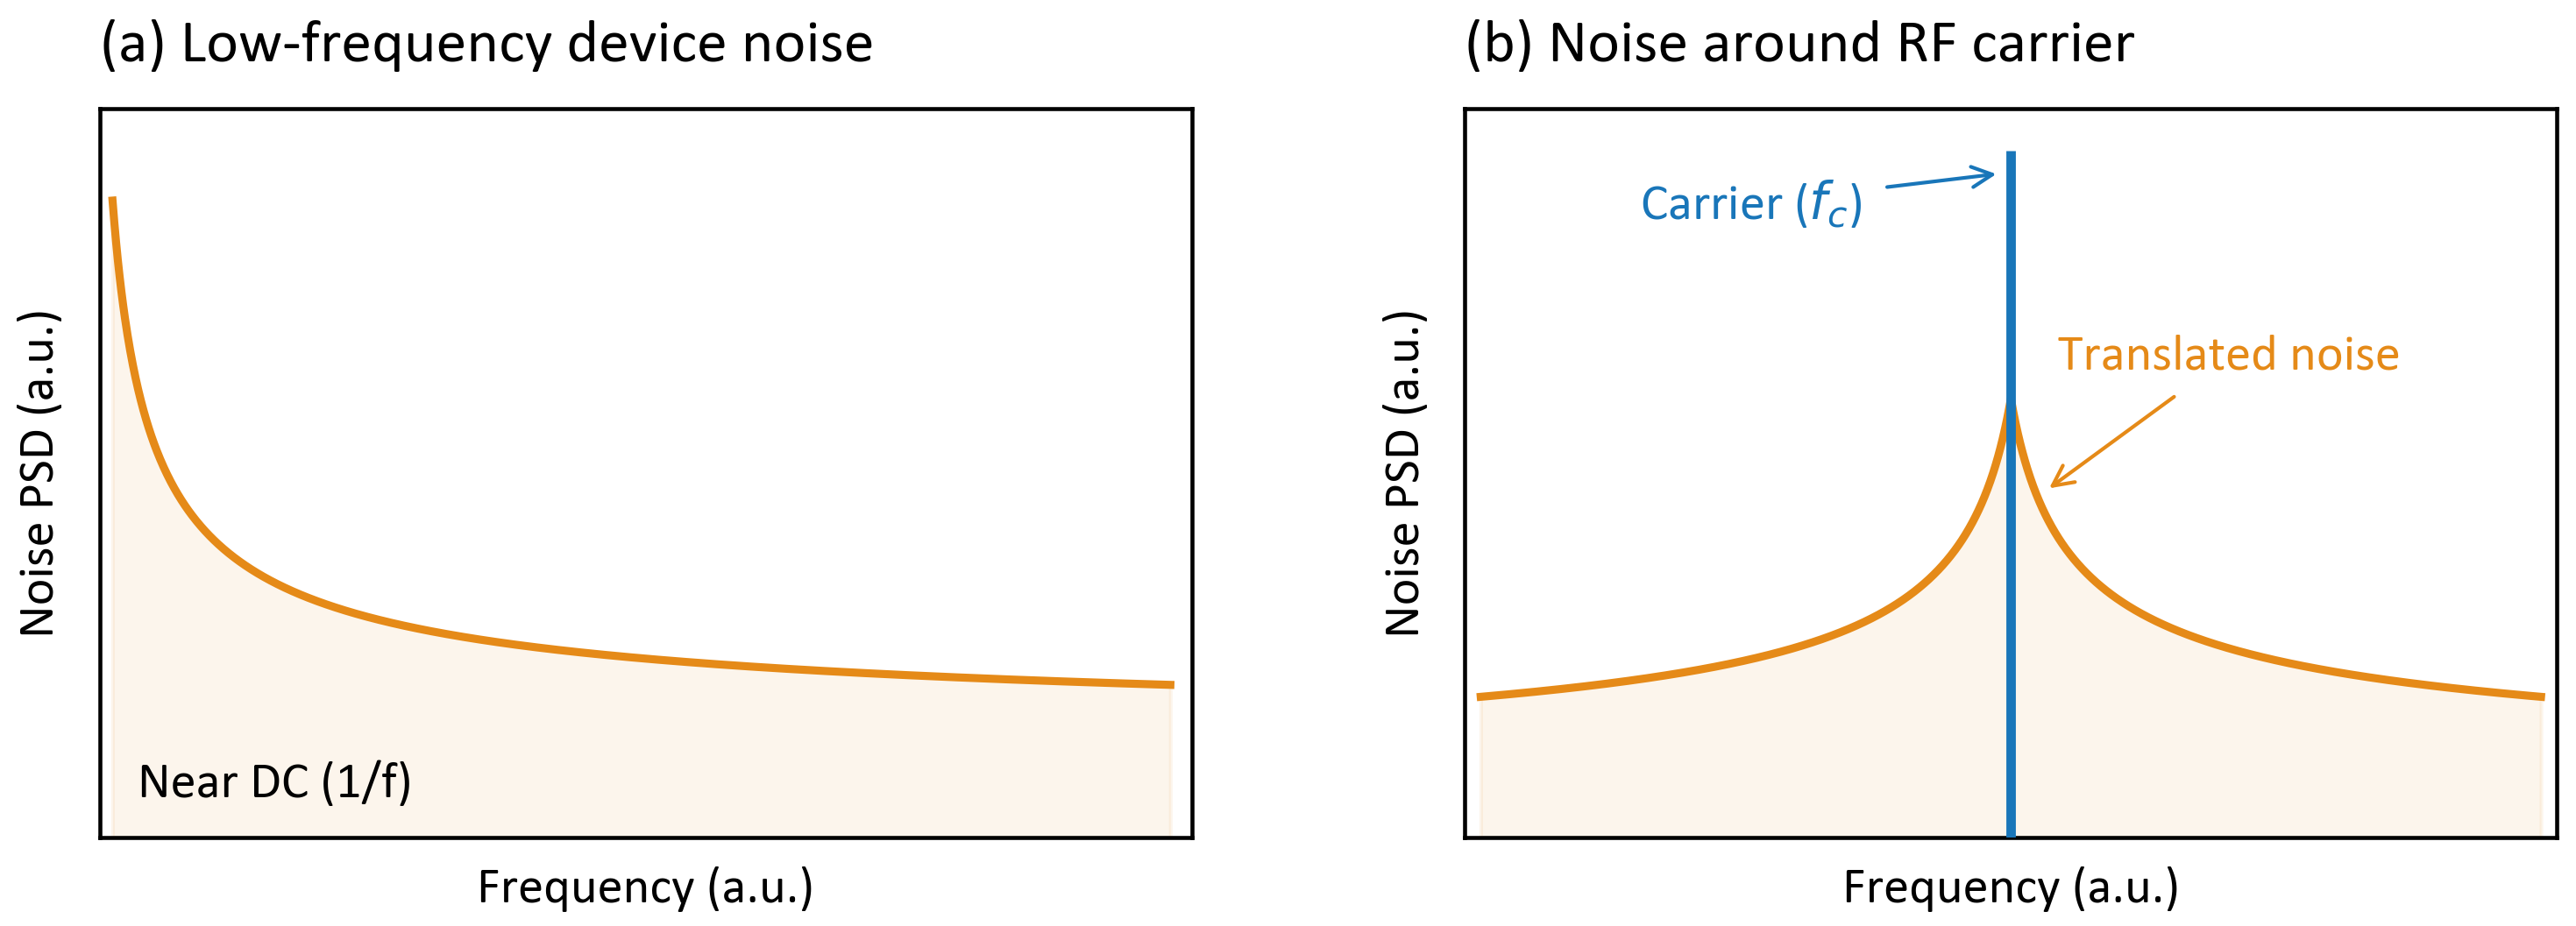
\includegraphics[width=0.9\linewidth]{figures/fig2.png}
		\caption{
			(a) Low-frequency device noise exhibiting a
			characteristic $1/f$-like spectrum near DC.
			(b) Sidebands around
			a high-frequency carrier due to upconversion. 
		}
		\label{fig:fig2}
	\end{figure}
	
	A noise-perturbed carrier can be expressed as
	
	\begin{equation}
		v(t) = [A_0 + a(t)]
		\cos\left(2\pi f_c t + \phi(t)\right),
	\end{equation}
	
	where $A_0$ and $f_c$ denote the nominal carrier
	amplitude and frequency, respectively, while $a(t)$
	and $\phi(t)$ represent noise-induced amplitude and
	phase fluctuations. Although these perturbations
	vary much more slowly than the carrier itself,
	they can generate spectral components in its
	immediate vicinity.
	
	The extent and nature of noise conversion depend
	strongly on the circuit topology and operating
	conditions. In oscillators, low-frequency device
	noise can contribute to close-in phase noise,
	whereas in mixers, periodically varying circuit
	behavior can translate noise between RF and
	baseband frequencies \cite{Darabi2000}.
	Consequently, identical device-level noise
	characteristics may produce substantially different
	effects depending on the circuit in which the
	device operates.

	
	
	
	
	\section{Phase Noise in Oscillators}
	
	One of the most significant consequences of flicker noise
	in RF oscillators is its contribution to close-in phase
	noise, which affects the spectral purity of the oscillating
	signal. Phase noise is commonly characterized by the
	single-sideband phase noise $\mathcal{L}(\Delta f)$,
	expressed in dBc/Hz, where $\Delta f$ denotes the frequency
	offset from the carrier.
	
	Flicker noise and white noise originating from active
	devices can perturb the instantaneous oscillation frequency,
	producing random phase fluctuations. Since phase represents
	the accumulated frequency deviation over time, their
	corresponding power spectral densities are related by
	
	\begin{equation}
		S_{\phi}(\Delta f) =
		\frac{S_{\delta f}(\Delta f)}{(\Delta f)^2},
	\end{equation}
	
	where $S_{\phi}$ and $S_{\delta f}$ denote the phase- and
	frequency-fluctuation power spectral densities, respectively.
	Thus, flicker-induced frequency fluctuations proportional
	to $1/\Delta f$ produce a $1/(\Delta f)^3$ phase-noise
	dependence, whereas white frequency noise produces a
	$1/(\Delta f)^2$ dependence.
	
	These behaviors can also be described using the classical
	Leeson model, which relates oscillator phase noise to
	the underlying noise sources and resonator characteristics
	\cite{Leeson1966}. A simplified Leeson-type expression,
	including an empirical flicker-noise contribution, is
	
	\begin{equation}
		\mathcal{L}_{\mathrm{lin}}(\Delta f)
		\propto
		\frac{F k_B T}{P_{\mathrm{osc}}}
		\left[1+\left(\frac{f_L}{\Delta f}\right)^2\right]
		\left[1+\frac{f_{\mathrm{flick}}}{\Delta f}\right],
	\end{equation}
	
	where $F$ is the effective noise factor, $k_B T$ the
	thermal-noise energy, and $P_{\mathrm{osc}}$ the oscillator
	signal power. The Leeson frequency $f_L=f_0/(2Q_L)$ depends
	on the oscillation frequency $f_0$ and loaded resonator
	quality factor $Q_L$, while $f_{\mathrm{flick}}$ represents
	an effective flicker-noise corner. The expression describes
	the approximate spectral behavior in linear units.
	
	Figure~\ref{fig:fig3} illustrates the characteristic
	phase-noise regions. At small frequency offsets,
	flicker-related frequency fluctuations produce a
	$1/(\Delta f)^3$ dependence ($-30$ dB/decade).
	Beyond the $1/f^3$ corner, white frequency noise
	typically produces a $1/(\Delta f)^2$ dependence
	($-20$ dB/decade), followed by a far-offset noise floor.
	This simplified sequence assumes that the flicker-related
	corner lies below the Leeson frequency.
	
	\begin{figure}[htbp]
		\centering
		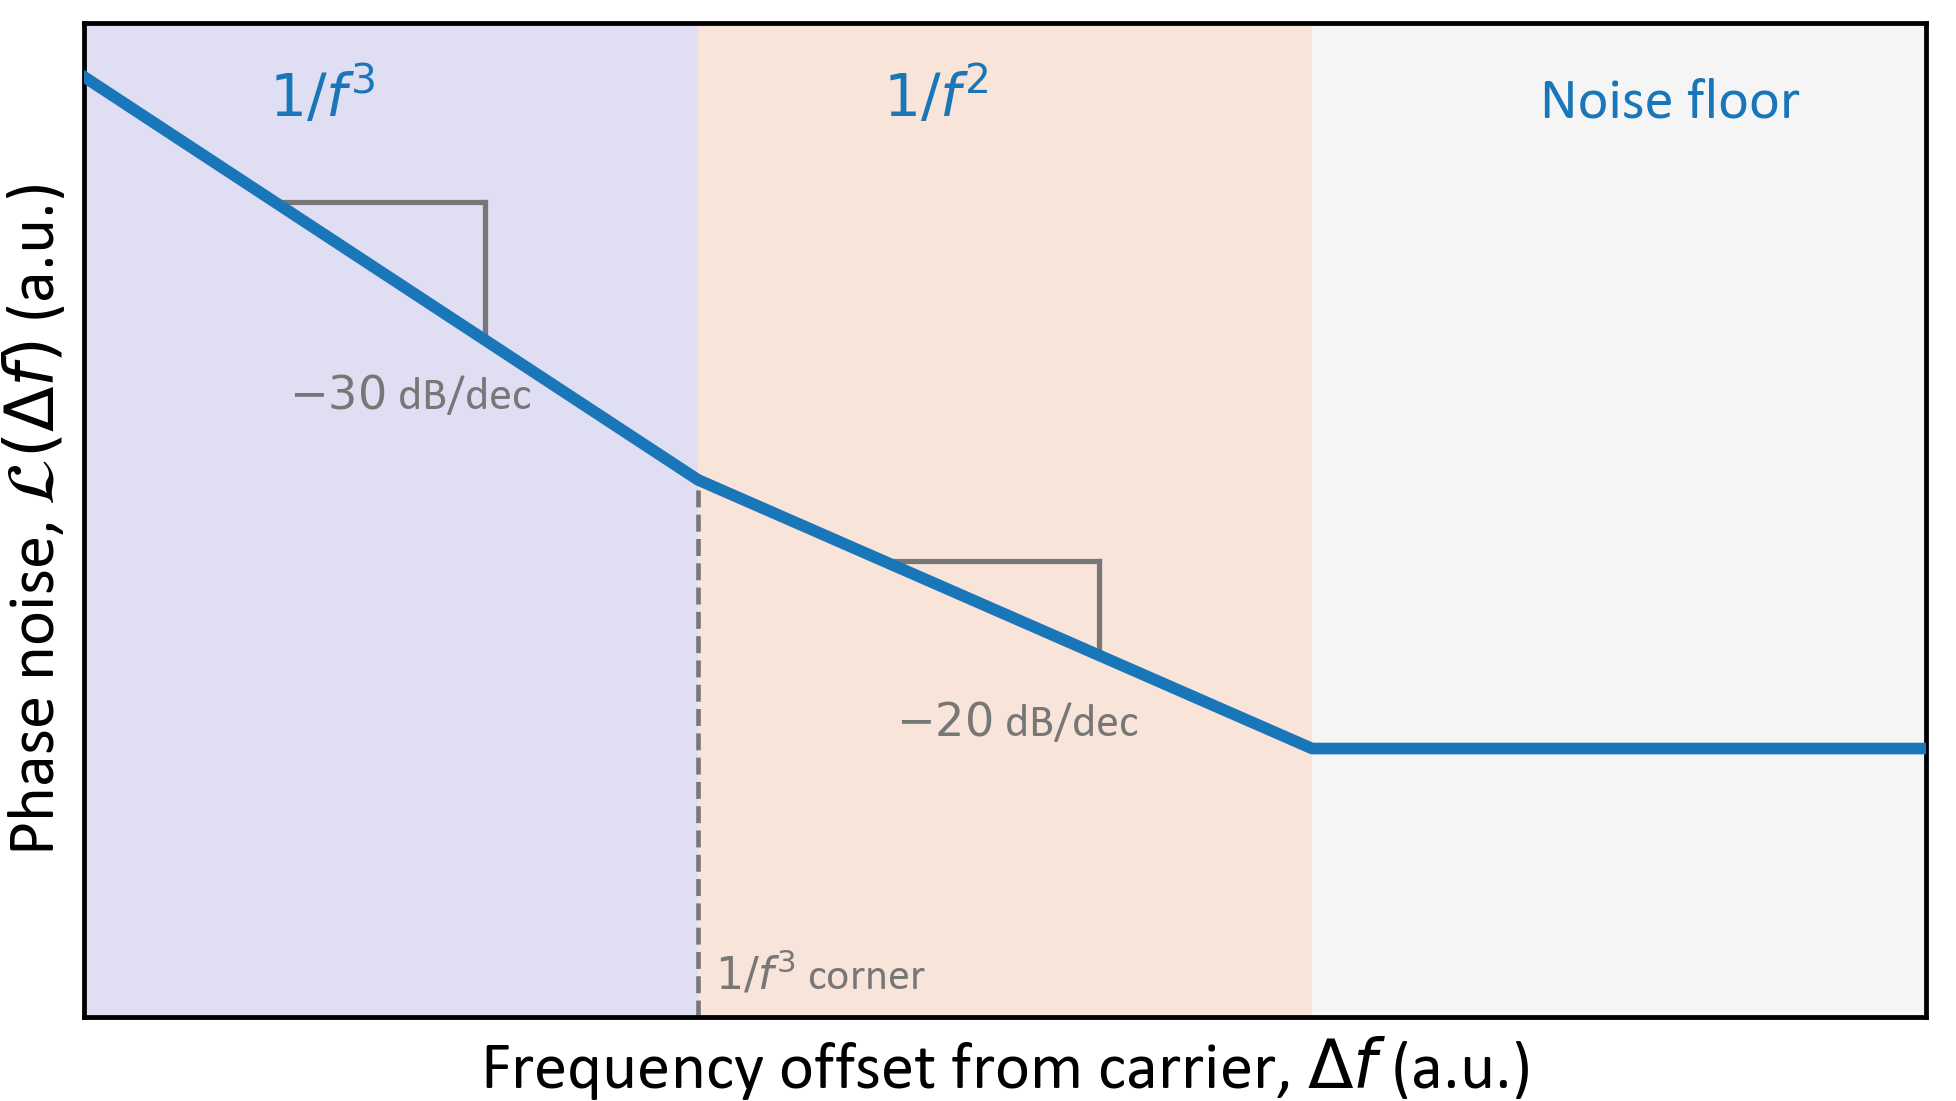
\includegraphics[width=0.55\linewidth]{figures/fig3.png}
		\caption{
			Conceptual RF oscillator phase-noise spectrum
			showing the $1/f^3$, $1/f^2$, and noise-floor
			regions, with the dashed line marking the
			$1/f^3$ corner.
		}
		\label{fig:fig3}
	\end{figure}
	
	The oscillator's $1/f^3$ corner is not
	necessarily identical to the intrinsic transistor
	flicker-noise corner, since noise conversion also
	depends on resonator properties and circuit topology.
	The oscillator's sensitivity to noise varies throughout
	each oscillation cycle, making the waveform and transistor
	conduction intervals important. Recent study on
	current-biased Class-B CMOS oscillators have shown that
	charge sharing between the tail capacitance and resonant
	tank during transistor triode operation can significantly
	enhance flicker-noise upconversion \cite{Bevilacqua2026}. Consequently, close-in phase noise depends not only
	on device-level flicker noise but also on oscillator
	architecture and operating conditions, highlighting
	the importance of accurate noise characterization
	for predicting RF oscillator performance.
	
	
	
	\section{Effect on Frequency Mixing}
	
	In RF mixers, local oscillators (LOs) are typically used
	to translate carrier signals between different frequency
	bands. As discussed previously, practical oscillators
	exhibit phase noise around their carrier frequency.
	During mixing, this phase noise is transferred to the
	converted signals, potentially affecting receiver
	performance.
	
	This effect becomes particularly important when multiple
	signals of different amplitudes are present at the receiver
	input. Ideally, each carrier would be translated to a
	discrete frequency at the intermediate-frequency (IF)
	output. However, the LO phase noise introduces spectral
	spreading around each converted carrier. The magnitude
	of these noise contributions depends on the respective
	carrier powers and the LO phase-noise characteristics
	\cite{Grebenkemper1981}.
	
	Figure~\ref{fig:fig4} illustrates this behavior using
	three input carriers, with the strongest located between
	two weaker signals. After frequency conversion, all
	three carriers exhibit phase-noise sidebands originating
	from the LO. Since the central carrier is significantly
	stronger, its associated noise contribution is also
	greater and extends over a wider frequency range before
	reaching the receiver's intrinsic noise floor. The
	weaker carrier on the left remains distinguishable,
	whereas the carrier on the right is nearly masked by
	the phase-noise contribution of the stronger carrier.
	
	\begin{figure}[htbp]
		\centering
		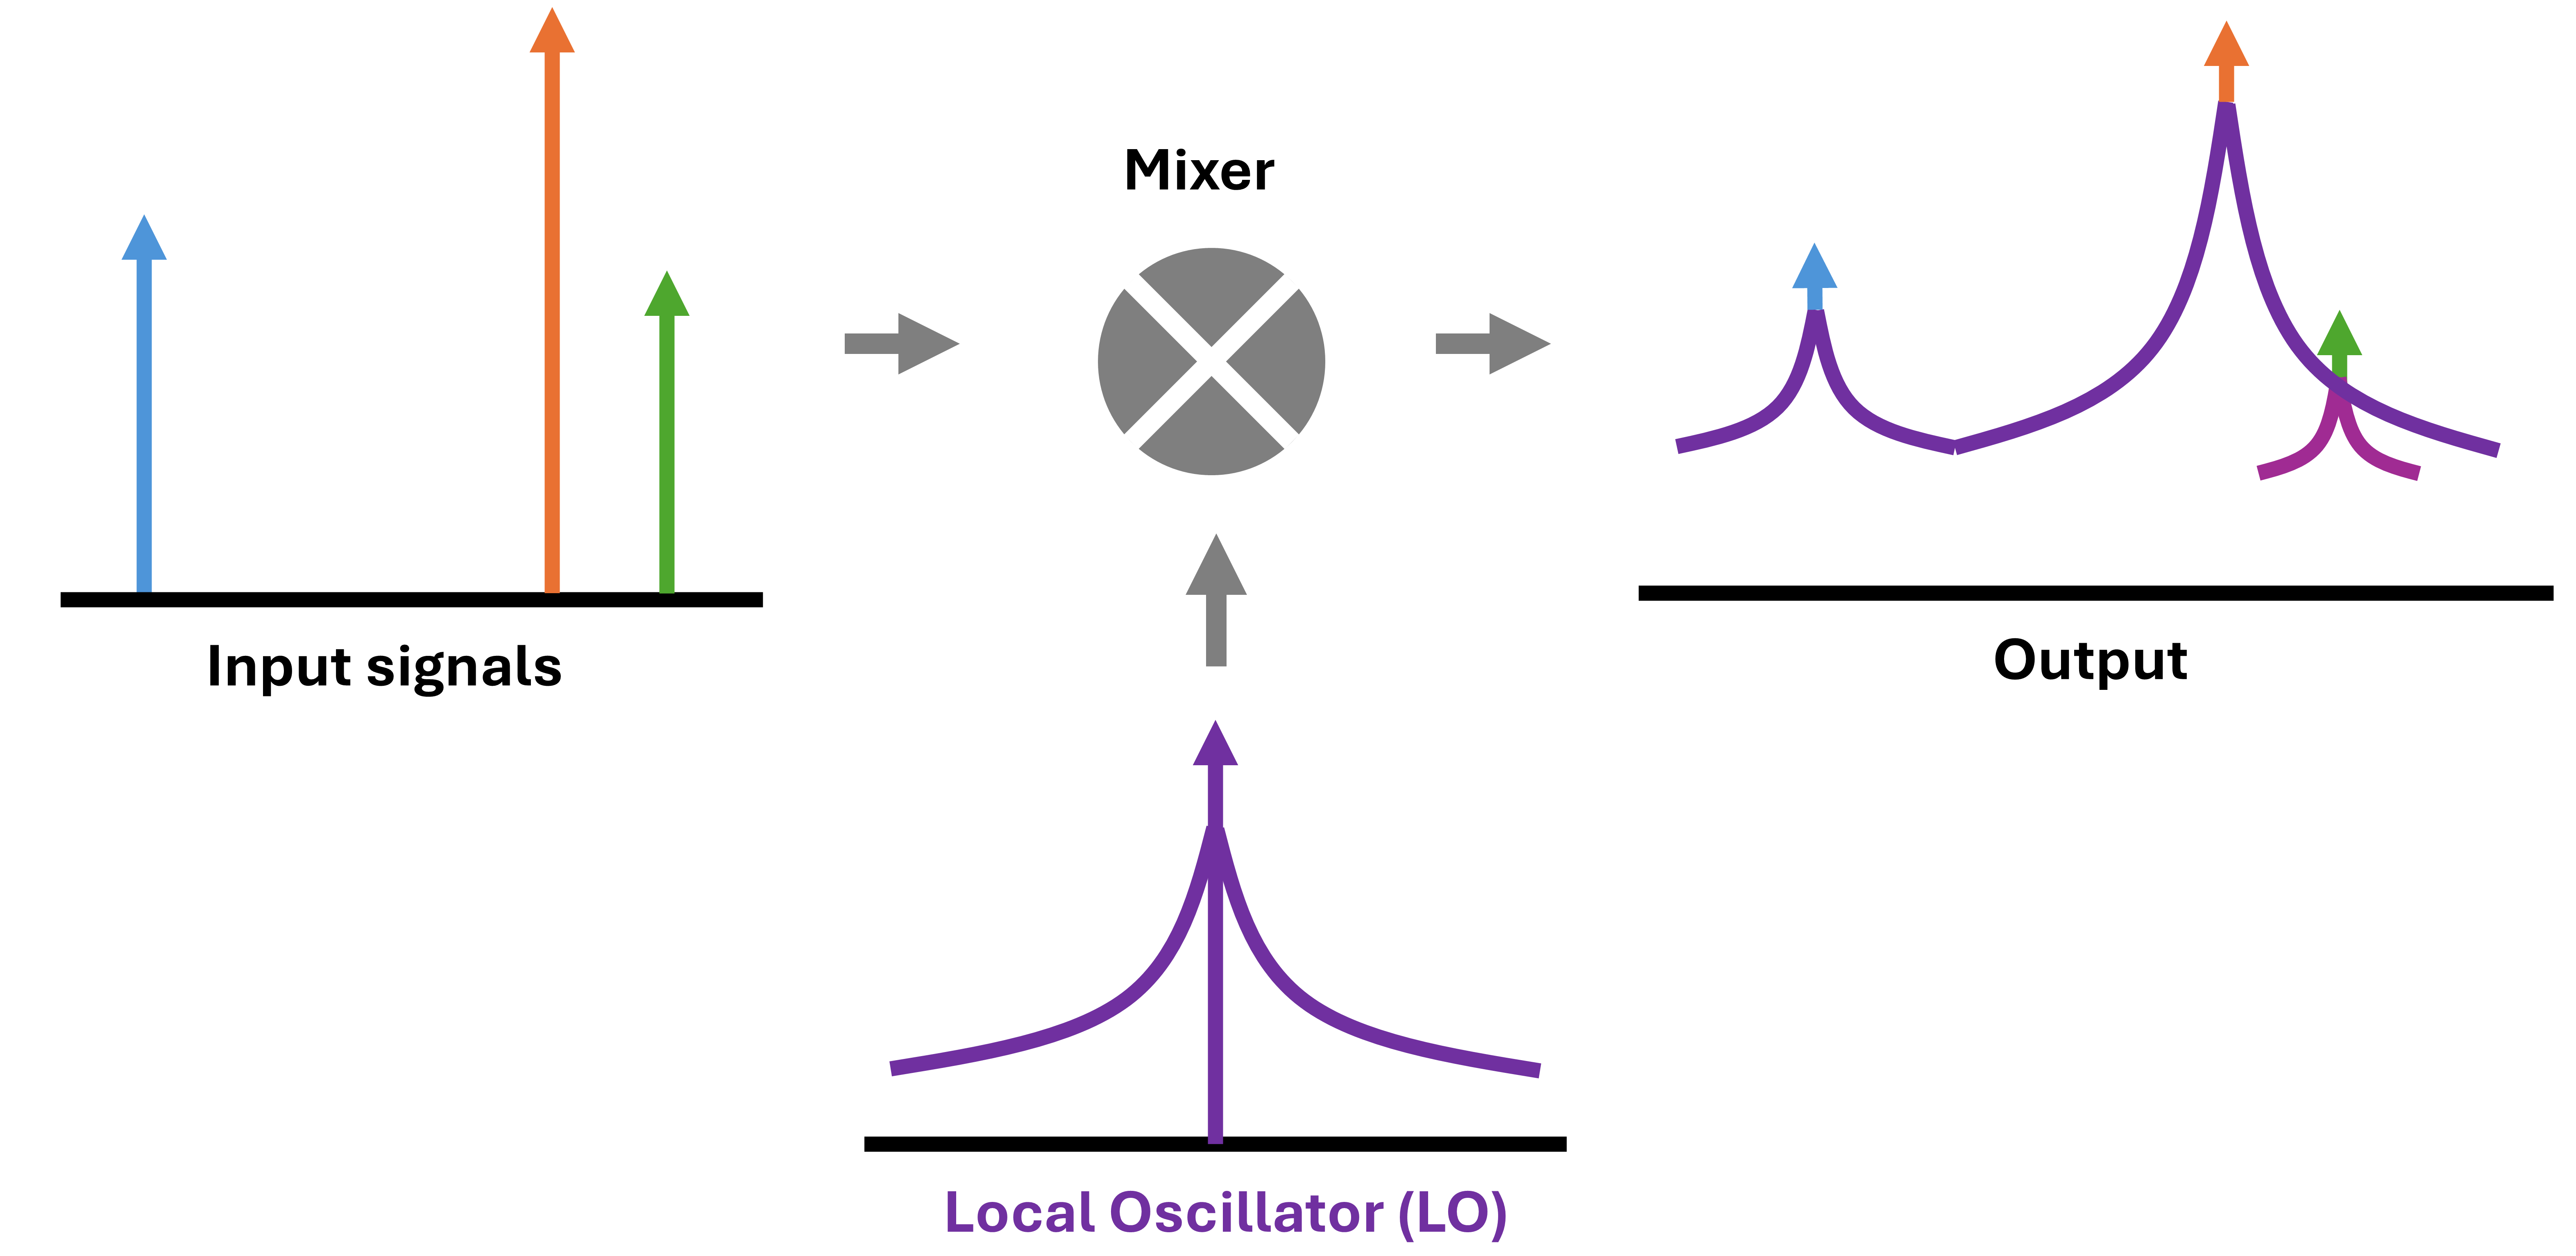
\includegraphics[width=0.65\linewidth]{figures/fig4.png}
		\caption{
			Illustration of reciprocal mixing, showing how
			LO phase noise from a strong carrier can mask
			weaker neighboring signals.
		}
		\label{fig:fig4}
	\end{figure}
	
	This phenomenon, known as \textit{reciprocal mixing},
	increases the apparent receiver noise floor near strong
	carriers. Consequently, a receiver tuned to a weaker
	neighboring signal may experience a significantly
	reduced signal-to-noise ratio (SNR), even when its
	intrinsic noise figure remains unchanged. The severity
	of this degradation depends on the carrier power and
	the LO phase noise at the corresponding frequency
	separation. Thus, flicker-noise-induced phase noise
	can ultimately limit receiver sensitivity and
	selectivity.
	
	
	\section{Conclusion}
	
	Low-frequency noise can influence RF circuit performance
	far beyond the frequency range in which it originates.
	Through nonlinear and time-varying circuit behavior,
	flicker noise can affect signal stability, spectral
	purity, and overall system performance. Its impact
	depends not only on the intrinsic noise characteristics
	of semiconductor devices but also on circuit topology
	and operating conditions. Understanding these effects
	and accurately characterizing device-level noise are
	therefore essential for developing high-performance
	RF circuits and communication systems.
	
	% ============================================================
	% REFERENCES
	% ============================================================
	
	\begin{thebibliography}{9}
		
		\bibitem{Hajimiri1998}
		A. Hajimiri and T. H. Lee,
		``A general theory of phase noise in electrical oscillators,''
		\textit{IEEE Journal of Solid-State Circuits},
		vol. 33, no. 2, pp. 179--194, Feb. 1998.
		doi: 10.1109/4.658619.
		
		\bibitem{Darabi2000}
		H. Darabi and A. A. Abidi,
		``Noise in RF-CMOS mixers: A simple physical model,''
		\textit{IEEE Journal of Solid-State Circuits},
		vol. 35, no. 1, pp. 15--25, Jan. 2000.
		doi: 10.1109/4.818916.
		
		\bibitem{Leeson1966}
		D. B. Leeson,
		``A simple model of feedback oscillator noise spectrum,''
		\textit{Proceedings of the IEEE},
		vol. 54, no. 2, pp. 329--330, Feb. 1966.
		doi: 10.1109/PROC.1966.4682.
		
		\bibitem{Bevilacqua2026}
		A. Bevilacqua and A. Mazzanti,
		``On the upconversion of the cross-coupled pair
		1/f noise into phase noise in current-biased
		Class-B CMOS oscillators,''
		\textit{IEEE Transactions on Circuits and Systems I:
			Regular Papers},
		vol. 73, no. 3, pp. 1777--1786, Mar. 2026.
		doi: 10.1109/TCSI.2025.3602924.
		
		\bibitem{Grebenkemper1981}
		C. J. Grebenkemper,
		``Local oscillator phase noise and its effect
		on receiver performance,''
		\textit{The Communications Edge},
		vol. 8, no. 6, Nov./Dec. 1981,
		reprinted by WJ Communications, 2001.
		
		
	\end{thebibliography}
	
\end{document}